\subsection{\textbf{RQ3:} Do developer tools meet practitioner needs for merge conflicts?}\label{RQ3}
Practitioners expect their merge tools to be easy to use, provide relevant information, and present that information in an understandable manner.
In order to understand which improvements practitioners value most, we asked interview participants open-ended questions about their merge conflict resolution process.

Our interviews informed the survey questions in which participants ranked 6 practitioner needs for tool improvements.
We received 119 responses using a 5-point Likert scale to indicate the usefulness each type of tool improvement (1 being \textit{Not Useful}, 3 being \textit{Moderately Useful}, and 5 being \textit{Essential}).

In addition, we also asked participants which tools they use during conflict resolution.
We received 105 different tools from 115 responses, though some were generic responses such as \textit{``my text editor''}.
We group these generic responses together where semantically similar meanings exist. 
Table~\ref{survey_toolset} lists the top 10 most common tools used by participants to resolve merge conflicts.

\begin{table}[!htbp]
\renewcommand{\arraystretch}{1.3}
\caption{Survey Participant Merge Toolsets (Top 10)}
\label{survey_toolset}
\centering
\begin{tabularx}{0.45\textwidth}{@{}r|Cl@{}}
\toprule
Tool & \# Participants & Description\\
\midrule
Git	& 37 & Version Control System\\
Vim/vi & 17 & Text Editor\\
Text Editor (unspecified) & 14 & Text Editor\\
Git Diff & 11 & Diffing Tool\\
GitHub & 11 & Website\\
Eclipse & 10 & IDE\\
KDiff3 & 9 & Diff \& Merge\\
Meld & 8 & Diff \& Merge\\
SourceTree & 8 & Git/Hg Desktop Client\\
Sublime Text & 7 & Text Editor\\
\bottomrule
\end{tabularx}
\end{table}

\subsubsection{\underline{Better Usability}}
The right toolset is essential for efficiently developing solutions and resolving conflicts.
Usability is a major factor that determines whether a toolset will support practitioner's workflows instead of hindering them.
Based on the results of the survey, we found that practitioners rate usability as the most desired improvement for their current merge tools (I1).

Usability within a particular tool is important, but these usability concerns also stretch across multiple tools that serve similar use cases and must operate in sync with each other.
Survey participants indicated that they use 2.5 tools on average, and as many as 7 tools, to resolve merge conflicts.
With multiple tools being used during merging and conflict resolution, toolset fragmentation is a real concern for practitioners.
For instance, during the interviews, P1 demonstrated resolving a typical merge conflict using four different tools and said: 
\begin{displayquote}
\textit{``I have to jump around between tools and copy and paste version numbers from one to... See, this is why [toolset] integration matters.''}
\end{displayquote}

This frustration is understandable for practitioners whose workflows frequently get interrupted by tool switches. Psychology studies~\cite{Meiran2000}\cite{gopher2000switching} have found that task switching comes with costs in performance and mental fatigue, and, in 1992, Gerald Weinberg highlighted the problem of toolset fragmentation within engineering teams~\cite{Weinberg1992}. 
This motivated a survey question asking, \textit{``How often do you find that having multiple tools has been a problem in your development workflow?''} We received 121 responses with a mean score of 2.04 (\textit{Rarely} on a 5-point Likert scale from \textit{Never} to \textit{Always}). 

In comparing the effect of toolsets on problems in development workflow, we recognize that issues with particular tools could bias practitioner perceptions.
Therefore, we examined the tool lists of participants that chose \textit{Never} or \textit{Rarely} against the tool lists of participants that chose \textit{Sometimes}, \textit{Often}, or \textit{Always} and found that these groups shared 9 out of 10 of the most common tools.
Since both groups are responding about problems in the same set of tools, we conclude that both groups had different perceptions about the difficulties in using multiple tools as opposed to their particular combination of tools.

\subsubsection{\underline{Better Filtering of Less-Relevant Information}}
Version control systems (VCS) and bug tracking systems provide insufficient support for detailed analysis of software evolution and information retrieval~\cite{fischer2003release_history}.
For software practitioners using \texttt{git} and other VCS, it is often easier to write scripts that accommodate their particular information needs by augmenting the capabilities of the VCS.
During the interviews, P1 described writing several scripts in order to locate particular historical commits that relate to a current merge conflict.
P9 also described a tool, \texttt{git-diff}, developed as part of their efforts to add additional difference analysis functionality across branches:
\begin{displayquote}
\textit{``git-diff will just do the diff based on the SHAs... we're adding metadata and cherry picking, so the SHAs are always going to be changing... this actually allows us to do a comparison based on SHA but then fall back to author and commit title and metadata information... It also hooks into GitHub labels and uses the labels on the project to do some more advanced heuristics.''}
\end{displayquote}
\todo{Shane: This transition is a bit rough}
In our survey results, we see that practitioners rank \textit{better ways of filtering out less relevant information} (I2) as the second highest improvement needed in modern merge toolsets.
Combined with our interviews, we find that the expansion of metadata capabilities in GitHub, GitLab\footnote{https://gitlab.com/}, and other cloud-based repository hosting services drives the development of scripts and tools to utilize this data in practitioners' workflows.
Further work is needed to bring these capabilities from single-purpose scripts into common toolsets used by all practitioners.

\subsubsection{\underline{Better Exploration of Project History}}
Codoban et al.~\cite{mihai_lenses} introduced the concept of the \textit{Archeology Lens} to describe examining old development history to retrieve lost knowledge and postulated that additional tool support was needed in this context.
We also find that practitioners consider history exploration to be a major area of improvement for development toolsets.
Among survey participants, \textit{better ways of exploring project history} (I3) ranked as the third most important improvement needed.
During our interviews, P1 said: 

\begin{displayquote}
\textit{``Give me a way to explore the history. To drill down, to go back up, you know? To resurface and understand what happened.''}
\end{displayquote}

The gap in support for analyzing development history among practitioner toolsets has previously been recognized by researchers~\cite{sun2015informationhistory, guo2016cold-start, yan2014miningcontracts}, however practical application of these efforts appear to have not yet reached practitioners.

\subsubsection{\underline{Better Graphical Presentation of Information}}
The usefulness of information is helped or hindered by the way in which it is presented to users.
In our survey results, we found that \textit{better graphical presentation of information} (I4) was ranked the fourth highest improvement needed in practitioner toolsets (mean: 3.14).
One of the survey participants' comment highlights this need for further toolset improvements:
\begin{displayquote}
\textit{``Tools don't make it easy to work with two arbitrary revisions side by side.''}
\end{displayquote}

In our interviews, several practitioners reported experiencing issues with inconsistent terminology, inconsistent visual metaphors (colors, notifications, etc.), and the organizational layout of different development tools.
The cost of context switching in software development is well-known to researchers~\cite{czerwinski2004taskswitching, li2007cost_of_context_switch, blackwell2002attentioninvestment, convertino2003dualview}, but the individual experiences of practitioners attempting to resolve merge conflicts isn't as well understood.
Practitioners conveyed that they would like to see tools that share a common language in both terminology and presentation, though survey participants indicated only a minor need for improvement in consistency of terminology. 

\begin{table}[!htbp]
\renewcommand{\arraystretch}{1.3}
\caption{Practitioners' Trust in their Merging, History Exploration, and Conflict Resolution Tools\textsuperscript{i}}
\label{survey_tool_trust}
\centering
\begin{tabularx}{0.45\textwidth}{@{}r|*{10}{C}c@{}}
\toprule
Trust Level & Response Count & Response \%\\
\midrule
Completely & 20 & 16.52\\
A lot & 50 & 41.32\\
A moderate amount & 41 & 33.88\\
A little & 10 & 8.26\\
Not at all & 0 & 0.00\\
\bottomrule
	\multicolumn{3}{c}{\noindent\parbox[t]{7.8cm}{\vspace{-3px}\textsuperscript{i}\hspace{0.2em}Survey respondents answered on a 5-point Likert scale to indicate trust in their toolset (1 being \textit{Not at all} and 5 being \textit{Completely}).}}
\end{tabularx}
\end{table}

\begin{figure*}[!htbp]
\centering
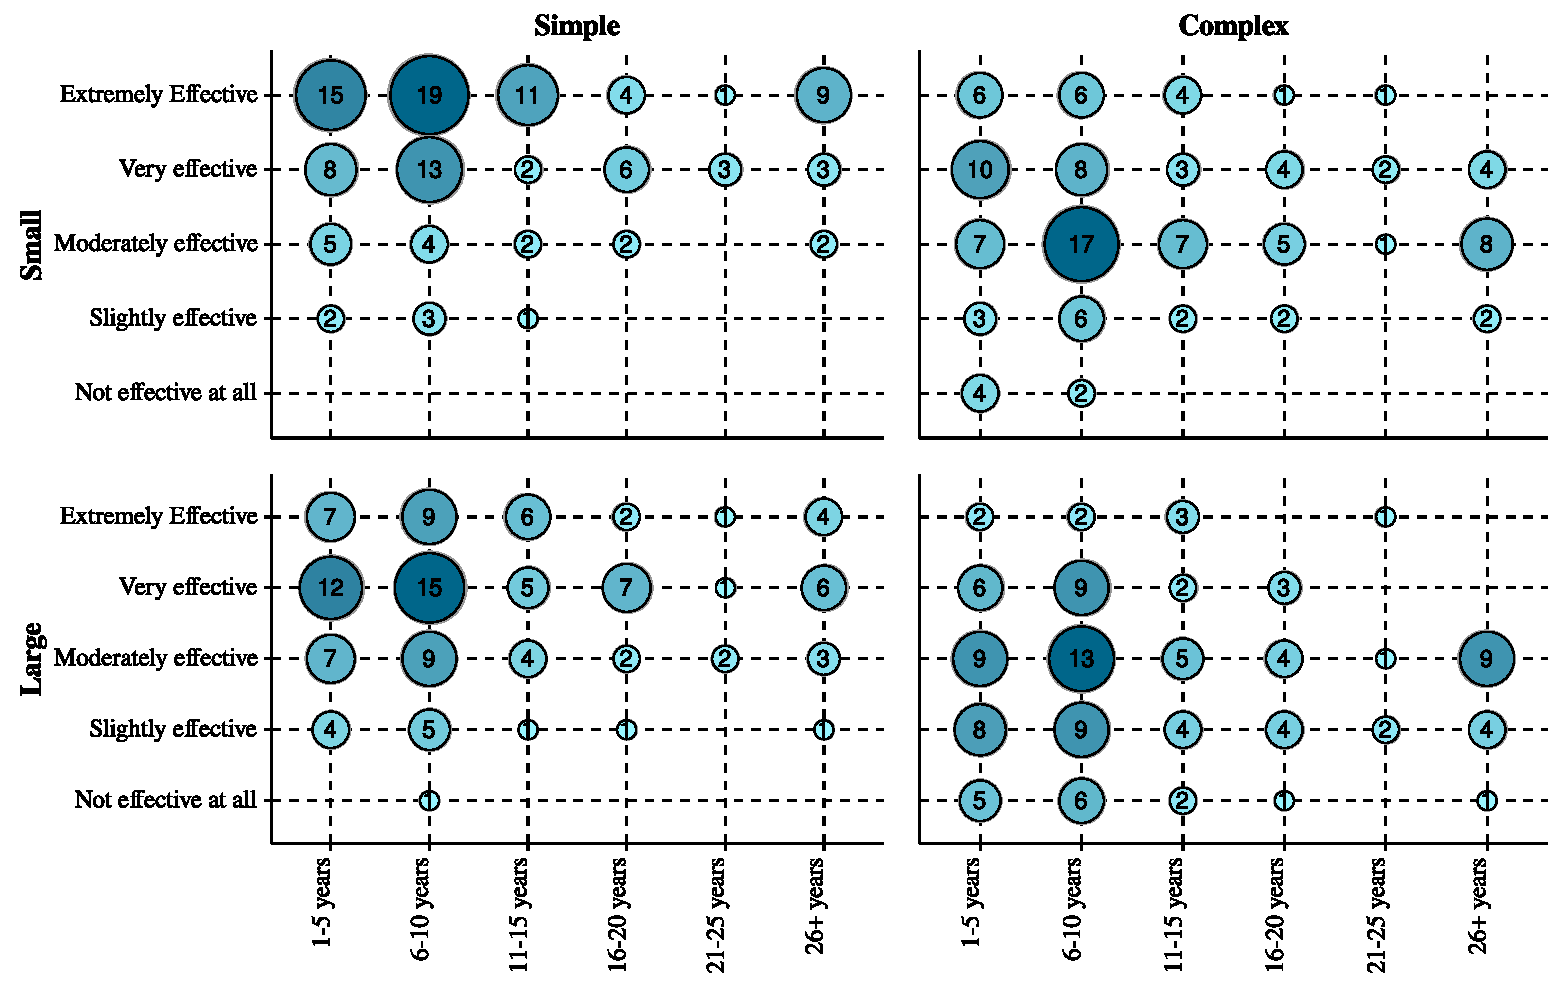
\includegraphics[width=\textwidth]{ConflictComplexityVsSize.pdf}
\caption{Effectiveness of practitioners' toolsets in supporting perceived size and complexity of merge conflicts, split on development experience. Bubble values indicate number of survey responses for effectiveness of a particular merge conflict size and complexity, and bubble size indicates the number of responses for comparison purposes.}
\label{size_vs_complexity}
\end{figure*}

\subsubsection{\underline{Tool Mistrust/Transparency}}
Most merge tools attempt to resolve conflicts using a variety of algorithms, but revert to manual resolution when these algorithms fail.
Several interview participants indicated that they mistrust merge tools when they obscure the steps and rationale for particular results when resolving merge conflicts.
The opaque nature of history exploration tools was also found to be a source of practitioners' overall mistrust of their toolsets.
P4 commented that:
\begin{displayquote}
\textit{``I've never trusted the merge tools, in a way. Or the diff tools. It would always just make me skittish. So my overall perception is that I'm scared of them. Sometimes I'll even manually go and do the merge myself rather than use a tool. Just because I've had several times where it's a bad merge, and I broke some code.''}
\end{displayquote}

Based upon this theme of mistrust, we asked survey participants to rate the degree to which they trust their merging, history exploration, and conflict resolution tools.
We received 121 responses to this question, with a mean score of 3.66 placing the most common responses between \textit{a moderate amount} and \textit{a lot} of trust (Table~\ref{survey_tool_trust}).
Assuming that responses of \textit{a moderate amount}, \textit{a little}, or \textit{not at all} indicate some degree of mistrust, we find that 42.15\% of practitioners experience some gap in toolset trust.

However, the severity of toolset mistrust is not as significant as the interview results had lead us to assume.
Only 8.26\% of practitioners indicated that they trust their toolset \textit{a little} or \textit{not at all} (10 out of 121 responses).
The results of the survey are counterintuitive to our interview results, but appears to indicate that practitioners abandon mistrusted tools before all trust is lost in them.

\subsubsection{\underline{Perceptions of Developer Tool Effectiveness}}
The perceived size and complexity of merge conflicts affect the way in which practitioners plan, allocate, and enact resolutions.
To understand the degree to which these two factors impact practitioners' perceptions about the effectiveness of their toolsets, we asked survey participants to rate their toolset across four different merge conflict archetypes: (1) \textit{simple, small merge conflicts}, (2) \textit{simple, large merge conflicts}, (3) \textit{complex, small merge conflicts}, and (4) \textit{complex, large merge conflicts}.

\todo{Shane: Is ''centrality'' a computeable metric? Might be better to chose another word, if it is.}
Since individual participants have different toolsets, and consider different factors when determining the perceived size and complexity of a merge conflict, we instructed participants to rate their own toolset against these archetypes using their own notion of what constitutes a simple vs. complex and small vs. large merge conflict.
Figure~\ref{size_vs_complexity} provides a visual illustration of the results of this survey question.

Observing the progression of results between each of the quadrants, we find that the centrality of results shifts from \textit{Extremely Effective} for \textit{small, simple merge conflicts} to \textit{Very Effective} for \textit{large, simple merge conflicts}.
This suggests that increasing the perceived size of a merge conflict has a slight affect on the perceived effectiveness of merge toolsets.
However, the shift from \textit{small, simple merge conflicts} to \textit{small, complex merge conflicts} shows a larger change in perceived effectiveness; from \textit{Extremely Effective} to \textit{Moderately effective}.

The results of this question indicate that modern merge tools are capable of handling an increase in perceived size of a merge conflict to a greater extend than an increase in the perceived complexity of a merge conflict.
We find this result to be hold true across each of the six software development experience groups.